\documentclass{amsart}
\usepackage{amsmath,amssymb,amsthm,fullpage,mathptmx, hyperref,dsfont,framed, graphicx, subcaption, textcomp} % The usual suspects

%%%%%%%%%%%%%%%%%% Tikz %%%%%%%%%
\usepackage{tikz}
\usetikzlibrary{shapes.geometric}
\usetikzlibrary{calc}
\usetikzlibrary{scopes}
\usetikzlibrary{decorations.markings}

\tikzset{
every picture/.style={line width=0.8pt, >=stealth,
                       baseline=-3pt,label distance=-3pt},
%%%%%%%%%%  Node styles
dotnode/.style={fill=black,circle,minimum size=2.5pt, inner sep=1pt, outer
sep=0},
morphism/.style={circle,draw,thin, inner sep=1pt, minimum size=15pt,
                 scale=0.8},
small_morphism/.style={circle,draw,thin,inner sep=1pt,
                       minimum size=10pt, scale=0.8},
coupon/.style={draw,thin, inner sep=1pt, minimum size=18pt,scale=0.8},
%%%% different line styles:
regular/.style={densely dashed},
edge/.style={thick, dashed, draw=blue, text=black},
boundary/.style={thick,  draw=blue, text=black},
overline/.style={preaction={draw,line width=2mm,white,-}},
drinfeld center/.style={>=stealth,green!60!black, double
distance=1pt,text=black},
%%%%%%% Fill styles %%%%%%%%%%%%%%%
cell/.style={fill=black!10},
subgraph/.style={fill=black!30},
%%%%%%% Mid-path arrows
midarrow/.style={postaction={decorate},
                 decoration={
                    markings,% switch on markings
                    mark=at position #1 with {\arrow{>}},
                 }},
midarrow/.default=0.5
}



\newtheorem{thm}{Theorem}[section]
\newtheorem*{uthm}{Theorem}
\newtheorem{lem}[thm]{Lemma}
\newtheorem*{ulem}{Lemma}
\newtheorem{prop}[thm]{Proposition}
%\newtheorem*{uprop}[thm]{Proposition}
\newtheorem{cor}[thm]{Corollary}
\newtheorem{conj}[thm]{Conjecture}
\newtheorem{defn}[thm]{Definition}
\newtheorem{rmk}[thm]{Remark}
\newtheorem{prob}[thm]{Open problem}
\newtheorem{ques}[thm]{Question}
\newtheorem{fact}[thm]{Fact}
\newtheorem{ex}[thm]{Exercise}


\DeclareMathOperator{\id}{id}
\DeclareMathOperator{\MCG}{MCG}
\DeclareMathOperator{\Mod}{Mod}
\DeclareMathOperator{\Vect}{Vec}
\DeclareMathOperator{\Homeo}{Homeo}
\DeclareMathOperator{\Hom}{Hom}
\DeclareMathOperator{\Obj}{Obj}
\DeclareMathOperator{\Irr}{Irr}
\DeclareMathOperator{\Img}{Im}
\DeclareMathOperator{\coev}{coev}
\DeclareMathOperator{\ev}{ev}



\begin{document}

\title{Finiteness for Mapping Class Group Representations from Twisted Dijkgraaf-Witten Theory}


\author{Paul Gustafson}
\email{pgustafs@math.tamu.edu}
\address{Department of Mathematics,
    Texas A\&M University,
    College Station, TX
    U.S.A.}
    

\begin{abstract}
Any twisted Dijkgraaf-Witten representation of a mapping class group of a closed surface has finite image.
\end{abstract}

\maketitle

\section{Introduction}
Given a spherical category $\mathcal A$ over a field $k$ and an oriented compact surface $M$, possibly with boundary, the Turaev-Viro construction gives a projective representation of the mapping class group $\MCG(M)$ \cite{TURAEV1992865, hep-th/9311155}.  A natural question is to determine the image of these representations.  In particular,  when does such a representation have finite image?

It is conjectured that these representations have finite image if and only if  $\mathcal A$ is weakly integral.  This conjecture is a modification of the Property F conjecture \cite{nr, erw}, which states that braid group representations coming from a braided monoidal category $\mathcal C$ should have finite image if and only if $\mathcal C$ is weakly integral.  Instead of only considering braid group representations, one can consider mapping class groups of arbitrary orientable surfaces.  In this case, the input categories to construct the representations must be more specialized than just braided monoidal.  One can either apply the Reshitikhin-Turaev construction to a modular tensor category, or apply the Turaev-Viro construction to a spherical category.  The former is more general than the latter since the the Reshitikhin-Turaev construction for the Drinfeld center $Z(\mathcal A)$ of a spherical category $\mathcal A$ yields the same representation as the Turaev-Viro construction for $\mathcal A$.  However, for the case considered in this paper, the simpler Turaev-Viro construction suffices.

% ^ Double check this ^ Does it work for any BMC?

In this paper, our input category is  $\mathcal A = \Vect_G^\omega$, the spherical category of $G$-graded vector spaces with associativity modified by a cocycle $\omega \in Z^3(G, k^\times)$.  In this case, the Turaev-Viro construction corresponds to the twisted Dijkgraaf-Witten theory of \cite{dijkgraaf1990}.  The category $\Vect_G^\omega$ is integral, so the one expects that its associated mapping class group representations have finite image.  Our main contribution is to verify this in the case  when the surface $M$ is closed and ($G$, $\omega$) are arbitrary.  

\textbf{Acknowledgments.}  This paper would not have been written without the guidance of my advisor, Eric Rowell.  I am also grateful to Zhengan Wang and my father Robert Gustafson for their advice.

\section{Related Work}

The closest related work is a result of Fjelstad and Fuchs \cite{fjfu} showing that, given a surface with at most one boundary component, the mapping class group representations corresponding to the untwisted (i.e. $\omega = 1$) Dijkgraaf-Witten theory have finite image.  Their paper uses an algebraic method of Lyubashenko \cite{Lyubashenko1996} that gives a projective mapping class group representation to any factorizable ribbon Hopf algebra, in their case, the double $D(G)$. In our case, we will considering the mapping class group action on a vector space of $\Vect_G^\omega$-colored embedded graphs defined by Kirillov \cite{kirillovStringNets}, yielding a simpler, more geometric proof.

In \cite{bantay}, Bantay defined representations of mapping class groups on the Hilbert space of an orbifold model associated to $D^\omega(G)$.  These representations appear to coincide with the twisted Dijkgraaf-Witten representations. However, the precise details of the connection are not clear to me.

More is known when we fix a particular surface $M$. In the case where $M$ is a torus, Ng and Schauenburg showed that any Reshitikhin-Turaev representation of the mapping class group of the torus is always finite \cite{0806.2493}.   In the case where $M$ is an $n$-punctured disk, the mapping class group of $M$ relative to the boundary of the disk is the braid group $B_n$.  In this case, Etingof, Rowell, and Witherspoon proved that the representations associated to $\Mod(D^\omega(G))$ are finite \cite{erw}.

\section{Definitions}

Let $M$ be a closed surface of genus $g$.  Let $G$ be a finite group, and let $\Vect_G^\omega$ denote the category of $G$-graded vector spaces with associativity defined by the  3-cocycle $\omega \in Z^3(G, k^\times)$.  More explicitly, we will follow \cite{math/0601012} in the choice of structural morphisms.  The associator $\alpha_{g,h,k}:(g \otimes h) \otimes k \to g \otimes (h \otimes k)$ is defined to be
$$\alpha_{g,h,k} = \omega(g,h,k) \id_{ghk}.$$ 
The evaluator $\ev_g:g^* \otimes g \to 1$ is 
$$\ev_g = \omega(g^{-1},g,g^{-1}) \id_1.$$  
The coevaluator $\coev_g:g \otimes g^* \to 1$ is 
$$\coev_g = \id_1.$$ 
The pivotal structure $j_g:g^{**} \to g$ is 
$$j_g = \omega(g^{-1},g,g^{-1}) \id_{g}.$$

\newcommand{\ee}{\mathbf{e}}       % oriented edge
\newcommand{\Ga}{\Gamma}
\newcommand{\ph}{\varphi}
\newcommand{\A}{\mathcal{A}}      % category 
\newcommand{\st}{\; | \;}                               %%  such that
\newcommand{\ttt}{\otimes}                              %% tensor product
\newcommand{\cc}[1]{\underset{\scriptstyle #1}{\circ}}
\newcommand{\ccc}[1]{\underset{\scriptstyle #1}{\bullet}}
\newcommand{\ti}{\tilde}
\newcommand{\ov}{\overline}
\newcommand{\del}{\partial}
\newcommand{\<}{\langle}
\renewcommand{\>}{\rangle}
\newcommand{\surjto}{\twoheadrightarrow}      %   -->> surjection
\newcommand{\injto}{\hookrightarrow}          %  (--> injection
\newcommand{\isoto}{\xrightarrow{\sim}}       % isomor.
\newcommand{\xxto}{\xrightarrow}              % long arrow
\newcommand{\firef}[1]{Figure~{\rm\ref{#1}}}
\newcommand{\R}{\mathbb{R}}       % real numbers

The following definitions and theorem are from Kirillov's paper
 \cite{kirillovStringNets}.
We will consider finite  graphs embedded in the surface $M$; for such a
graph $\Ga$, let $E(\Ga)$ be the set of edges. Note that edges are not
oriented. Let $E^{or}$ be the set of oriented edges, i.e. pairs $\ee=(e,
\text{orientation of } e)$; for such an oriented edge $\ee$, we denote by
$\bar{\ee}$ the edge with opposite orientation.

\begin{defn}\label{d:coloring} Let  $\Ga \subset M$ be an embedded graph as
defined above.  A {\em coloring} of $\Ga$ is the
following data:

  \begin{itemize}
    \item Choice of an object $V(\ee)\in \Obj \A$ for every oriented edge
        $\ee\in E^{or}(\Ga)$ so that $V(\ov{\ee})=V(\ee)^*$.
    \item Choice of a vector $\ph(v)\in \Hom (1, V(\ee_1) \otimes \dots \otimes V(\ee_n))$  for    every interior vertex $v$, where 
      $\ee_1, \dots, \ee_n$ are edges incident to $v$, taken in counterclockwise 
      order and with outward orientation. 
\end{itemize}
\end{defn}


The following theorem is a variation of result of Reshetikhin and Turaev. 
\begin{thm}\label{t:RT}
  There is a unique  way to assign to every colored
  planar graph $\Ga$ in a disk $D\subset \R^2$ a vector
  \begin{equation}
    \<\Ga\>_D\in \Hom (1, V(\ee_1) \otimes \dots \otimes V(\ee_n))
  \end{equation}
  where $\ee_1,\dots, \ee_n$ are the edges of $\Ga$ meeting the boundary
  of $D$ (legs), taken in counterclockwise order and with outgoing orientation,
  so that that following conditions are satisfied:
  \begin{enumerate}
     \item $\<\Ga\>$ only depends on the isotopy  class of $\Ga$.

    \item If $\Ga$ is a single vertex colored by
          $\ph\in \Hom (1, V(\ee_1) \otimes \dots \otimes V(\ee_n))$, then $\<\Ga\>=\ph$.
     
    \item Local relations shown in \firef{f:local_rels1} hold. 



\begin{figure}[ht]
%%%%%%%%%%%%%%%%%%%%%%%%%%%%%%%%%%%%%%%%%%%%%%%%%%%%%%%
%%%%%%%%%%
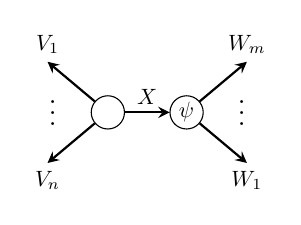
\begin{tikzpicture}
\node[morphism] (ph) at (0,0) {$\ph$};
\node[morphism] (psi) at (1,0) {$\psi$};
\node at (-0.7,0.1) {$\vdots$};
\node at (1.7,0.1) {$\vdots$};
\draw[->] (ph)-- +(220:1cm) node[pos=1.0,below,scale=0.8]
{$V_n$};
\draw[->] (ph)-- +(140:1cm) node[pos=1.0,above,scale=0.8]
{$V_1$};
\draw[->] (psi)-- +(40:1cm) node[pos=1.0,above,scale=0.8]
{$W_m$};
\draw[->] (psi)-- +(-40:1cm) node[pos=1.0,below,scale=0.8]
{$W_1$};
\draw[->] (ph) -- (psi) node[pos=0.5,above,scale=0.8] {$X$};
\end{tikzpicture}
%%%%%%%%
=
%%%%%%%%
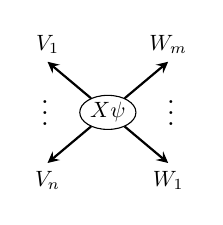
\begin{tikzpicture}
\node[ellipse, thin, scale=0.8, inner sep=1pt, draw] (ph) at (0,0)
             {$\ph\cc{X}\psi$};
\node at (-0.8,0.1) {$\vdots$};
\node at (0.8,0.1) {$\vdots$};
\draw[->] (ph)-- +(220:1cm) node[pos=1.0,below,scale=0.8] {$V_n$};
\draw[->] (ph)-- +(140:1cm) node[pos=1.0,above,scale=0.8] {$V_1$};
\draw[->] (ph)-- +(40:1cm) node[pos=1.0,above,scale=0.8]  {$W_m$};
\draw[->] (ph)-- +(-40:1cm) node[pos=1.0,below,scale=0.8] {$W_1$};
\end{tikzpicture}
%%%%%%%%%
\\
%%%%%%%%%
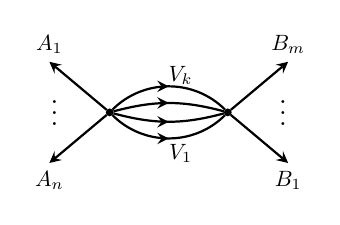
\begin{tikzpicture}
\node[dotnode] (ph) at (0,0) {};
\node[dotnode] (psi) at (1.5,0) {};
\node at (-0.7,0.1) {$\vdots$};
\node at (2.2,0.1) {$\vdots$};
\draw[->] (ph)-- +(220:1cm) node[pos=1.0,below,scale=0.8] {$A_n$};
\draw[->] (ph)-- +(140:1cm) node[pos=1.0,above,scale=0.8] {$A_1$};
\draw[->] (psi)-- +(40:1cm) node[pos=1.0,above,scale=0.8] {$B_m$};
\draw[->] (psi)-- +(-40:1cm) node[pos=1.0,below,scale=0.8] {$B_1$};
\draw[out=45,in=135, midarrow] (ph) to (psi)
                node[above,xshift=-0.6cm, yshift=0.25cm, scale=0.8] {$V_k$};
\draw[ out=15,in=165, midarrow] (ph) to (psi);
\draw[ out=-15,in=195, midarrow] (ph) to (psi);
\draw[ out=-45,in=225, midarrow] (ph) to (psi) node[below, xshift=-0.6cm, yshift=-0.3cm, scale=0.8] {$V_1$};
\end{tikzpicture}
%%%%%%%%%%%
=
%%%%%%%%%%%
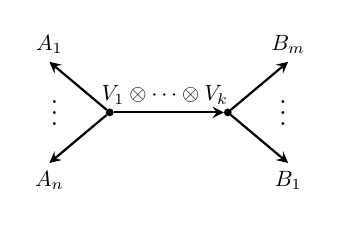
\begin{tikzpicture}
\node[dotnode] (ph) at (0,0) {};
\node[dotnode] (psi) at (1.5,0) {};
\node at (-0.7,0.1) {$\vdots$};
\node at (2.2,0.1) {$\vdots$};
\draw[->] (ph)-- +(220:1cm) node[pos=1.0,below,scale=0.8] {$A_n$};
\draw[->] (ph)-- +(140:1cm) node[pos=1.0,above,scale=0.8] {$A_1$};
\draw[->] (psi)-- +(40:1cm) node[pos=1.0,above,scale=0.8] {$B_m$};
\draw[->] (psi)-- +(-40:1cm) node[pos=1.0,below,scale=0.8] {$B_1$};
\draw[ ->] (ph) to (psi)
            node[above,xshift=-0.8cm,scale=0.8] {$V_1\otimes \dots\otimes V_k$};
\end{tikzpicture}
%%%%%%%
\qquad $k\ge 0$\\
%%%%%%%
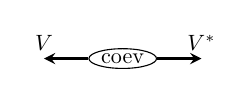
\begin{tikzpicture}
\node[ellipse, scale=0.8, inner sep=1pt, draw,thin] (ph) at (0,0)
{$\coev$};
\draw[->] (ph)-- +(180:1cm) node[pos=1.0,above,scale=0.8] {$V$};
\draw[->] (ph)-- +(0:1cm) node[pos=1.0,above,scale=0.8] {$V^*$};
\end{tikzpicture}
%%%%%%%%
=
%%%%%%%%
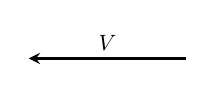
\begin{tikzpicture}
\draw[->] (2,0)-- (0,0) node[pos=0.5,above,scale=0.8] {$V$};
\end{tikzpicture}
%%%%%%%%%%%%%%%%%%%%%%%%%%
\caption{Local relations for colored graphs.
  Here $\ph\cc{X}\psi =  (\ph \otimes \psi) \circ \ev_X$. 
        }\label{f:local_rels1}
\end{figure}

    Local relations should be understood as follows: for any pair 
    $\Ga, \Ga'$ of colored graphs which are identical  outside a subdisk 
	$D'\subset D$, and in this disk are homeomorphic to the graphs
    shown in  \firef{f:local_rels1},  we must have $\<\Ga\>=\<\Ga'\>$. 
   \end{enumerate}
    Moreover, so defined $\<\Ga\>$ satisfies the following properties:
    \begin{enumerate} 
    \item $\<\Ga\>$ is linear in color of each vertex $v$ \textup{(}for 
         fixed colors of edges and other vertices\textup{)}.
    \item $\<\Ga\>$ is additive in colors of edges as shown in 
          \firef{f:linearity}.
\begin{figure}[ht]
$$
%%%%%%%%%%%%
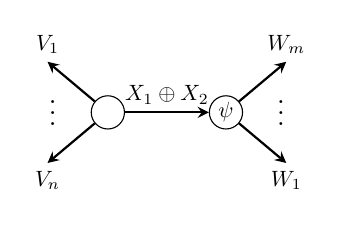
\begin{tikzpicture}
\node[morphism] (ph) at (0,0) {$\ph$};
\node[morphism] (psi) at (1.5,0) {$\psi$};
\node at (-0.7,0.1) {$\vdots$};
\node at (2.2,0.1) {$\vdots$};
\draw[->] (ph)-- +(220:1cm) node[pos=1.0,below,scale=0.8] {$V_n$};
\draw[->] (ph)-- +(140:1cm) node[pos=1.0,above,scale=0.8] {$V_1$};
\draw[->] (psi)-- +(40:1cm) node[pos=1.0,above,scale=0.8] {$W_m$};
\draw[->] (psi)-- +(-40:1cm) node[pos=1.0,below,scale=0.8] {$W_1$};
\draw[->] (ph) -- (psi) node[pos=0.5,above,scale=0.8] {$X_1\oplus X_2$};
\end{tikzpicture}
%%%%%%%%%%%%
=
%%%%%%%%%%%%
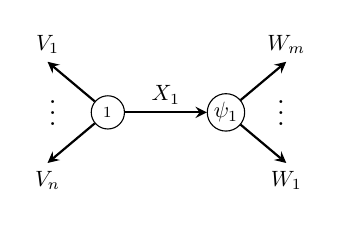
\begin{tikzpicture}
\node[morphism] (ph) at (0,0) {$\ph_1$};
\node[morphism] (psi) at (1.5,0) {$\psi_1$};
\node at (-0.7,0.1) {$\vdots$};
\node at (2.2,0.1) {$\vdots$};
\draw[->] (ph)-- +(220:1cm) node[pos=1.0,below,scale=0.8]{$V_n$};
\draw[->] (ph)-- +(140:1cm) node[pos=1.0,above,scale=0.8]{$V_1$};
\draw[->] (psi)-- +(40:1cm) node[pos=1.0,above,scale=0.8]{$W_m$};
\draw[->] (psi)-- +(-40:1cm) node[pos=1.0,below,scale=0.8]{$W_1$};
\draw[->] (ph) -- (psi) node[pos=0.5,above,scale=0.8] {$X_1$};
\end{tikzpicture}
%%%%%%%%%%%%
+
%%%%%%%%%%%%
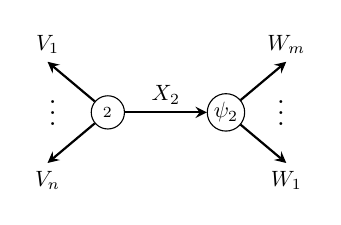
\begin{tikzpicture}
\node[morphism] (ph) at (0,0) {$\ph_2$};
\node[morphism] (psi) at (1.5,0) {$\psi_2$};
\node at (-0.7,0.1) {$\vdots$};
\node at (2.2,0.1) {$\vdots$};
\draw[->] (ph)-- +(220:1cm) node[pos=1.0,below,scale=0.8]{$V_n$};
\draw[->] (ph)-- +(140:1cm) node[pos=1.0,above,scale=0.8]{$V_1$};
\draw[->] (psi)-- +(40:1cm) node[pos=1.0,above,scale=0.8]{$W_m$};
\draw[->] (psi)-- +(-40:1cm) node[pos=1.0,below,scale=0.8]{$W_1$};
\draw[->] (ph) -- (psi) node[pos=0.5,above,scale=0.8] {$X_2$};
\end{tikzpicture}
%%%%%%%%%%%%
$$
\caption{Linearity of $\<\Ga\>$. Here $\ph_1,\ph_2$ are compositions
of $\ph$ with projector $X_1\oplus X_2\to X_1$ (respectively, 
$X_1\oplus X_2\to X_2$), and similarly for $\psi_1,\psi_2$.
}\label{f:linearity}
\end{figure}
    
    \item Composition property: if $D'\subset D$ is a subdisk such
      that $\del D'$ does not contain vertices of $\Ga$ and meets edges of
      $\Ga$ transversally, then   $\<\Ga\>_D$ will not change if we replace
      subgraph $\Ga\cap D'$ by a single vertex colored by
      $\<\Ga\cap D'\>_{D'}$.

  \end{enumerate}
The vector $\<\Ga\>$ is called the {\em evaluation} of $\Ga$.
\end{thm}

To define local relations between graphs, Kirillov defines the space of
null graphs as follows.  Let $D\subset M$ be an embedded disk, and let
$\Ga=c_1\Ga_1+\dots+c_n\Ga_n$ be a linear
combination of colored graphs in $M$ such that
\begin{enumerate}
  \item $\Ga$ is transversal to $\del D$ (i.e., no vertices of $\Ga_i$ 
      are on the boundary of $D$ and edges of each $\Ga_i$ meet 
      $\del D$ transversally).
  \item All $\Ga_i$ coincide outside of $D$.
  \item $\<\Ga\>_D=\sum c_i\<\Ga_i\cap D\>_D=0$.
\end{enumerate}
In this case $\Ga$ is called a null graph. 

\begin{defn}
The representation space $H$ is the vector space of formal linear combinations of $\Vect_G^\omega$-colored graph embeddings modulo the subspace spanned by the null graphs.
\end{defn}
%% The action of the mapping class group on H

\section{Result}

%% \begin{prop}
%% The action of the mapping class group on the vector space $H$ induced by the action of the orientation-preserving homeomorphisms on the surface $M$ is well-defined.
%% \end{prop}
%% \begin{proof}
%% The orientation-preserving group $\Homeo^+(M)$ acts on colored embedded graphs in $M$.  To see that the mapping class group $\MCG(M)$ has a well-defined action on $H$, we need to check two things: first, that isotopic homeomorphisms acting on a colored graph take it to equivalent colored graphs and, second, that a homeomorphism maps equivalent colored graphs to equivalent colored graphs.

%% For the first, suppose $f, g \in Homeo^+(M)$ are isotopic, with $H: M \times I \to M$ an isotopy from $f$ to $g$.  Let $i: \Gamma \to M$ be an graph embedding.  Then $H \circ i$ is an isotopy from $f \circ i$ to $g \circ i$.    

%% For the second,  to check that a homeomorphism $f \in \Homeo^+(M)$ preserves equivalence of colored graphs, it suffices to check that it in the case of each local move.  Since the mapping class group is generated by Dehn twists, all the local moves reduce to the isotopy move. 

%% To check that isotopic colored graphs get mapped to equivalent colored graphs, suppose $\Gamma$ is a graph and $i: \Gamma to M$ and $j: \Gamma \to M$ are isotopic embeddings. Let $H: \Gamma \times I \to M$ be an isotopy from $i$ to $j$.  Let $f \in \Homeo^+(M)$.  Then $f \circ H$ is an isotopy from $f \circ i$ to $f \circ j$.  

%% Thus, the action of the mapping class group on $H$ is well-defined.
%% \end{proof}




\begin{thm}
The image of the twisted Dijkgraaf-Witten representation of a mapping class group of any closed surface $M$ is finite.
\end{thm}

\begin{proof}
Let $\Gamma$ be a $\Vect_G^\omega$-colored graph embedding, and let $n$ be the genus of $M$ . Thinking of $M$ as a quotient of its fundamental $4n$-gon, by isotopy we may assume vertices of $\Gamma$ lie in the interior of the polygon and that all the edges of $\Gamma$ do not intersect corners and meet the sides transversally.  Evaluating on the interior of the polygon shows that $\Gamma$ is equivalent to a graph with a single vertex whose edges are simple closed curves, each of which intersect the boundary of the polygon precisely once.  By using the local relations, we can replace all the edges intersecting a side with a single edge labeled by the tensor product of their labels.  If there are no edges intersecting a side, we can insert a single edge labeled by the group identity into $\Gamma$ that intersects only that side.  Thus, $\Gamma$ is equivalent to a colored graph with one vertex $v$, outgoing edges $e_1, \ldots, e_{2n}$, and $2n$ incoming edges with the same labels as in Figure \ref{fig:span}.

By the definition of the evaluation of a string-net and the definition of the quotient map identifying the sides of the fundamental polygon, the vertex $v$ is colored by an element $\phi(v) \in \Hom (1, \bigotimes_{i=1}^n V(e_{2i-1}) \otimes V(e_{2i})  \otimes V(e_{2i-1}^*) \otimes V(e_{2i}^*))$, where $V(e_i) \in \Obj(\Vect_G^\omega)$ is the coloring of the edge $e_i$.  Since string-net evaluation is additive in the direct sum and linear in the vertex color, it follows that $H$ is spanned by the set of colored graphs
$$ S := \{\Gamma \in H : V(e_i) \in \Irr(\Vect_G^\omega), \phi(v) = 1 \}, $$
where $\Irr(\Vect_G^\omega)$ is the set of simple objects of $\Vect_G^\omega$, which correspond to the elements of $G$. 

\newdimen\R
\R=0.8cm

\begin{figure}

    \begin{tikzpicture}[scale=3]    

      \draw (0:\R) \foreach \x in {45,90,...,359} {
                -- (\x:\R)
            } -- cycle;
      
                 
    \begin{scope}[very thick,decoration={
    markings,
    mark=at position 0.5 with {\arrow{>}}}
    ]  
      \draw[postaction={decorate}]  (0, 0) --  (22: {0.923879*\R}) node[pos=.5,sloped,above]{$g$};
      \draw[postaction={decorate}]  (0, 0) --  (67: {0.923879*\R}) node[pos=.5,sloped,above]{$h$};
      \draw[postaction={decorate}]  (112: {0.923879*\R}) -- (0, 0) node[pos=.5,sloped,above]{$g$};
      \draw[postaction={decorate}]  (157: {0.923879*\R}) -- (0, 0) node[pos=.5,sloped,above]{$h$};
      \draw[postaction={decorate}]  (0, 0) --  (202: {0.923879*\R}) node[pos=.5,sloped,above]{$k$};
      \draw[postaction={decorate}]  (0, 0) --  (247: {0.923879*\R}) node[pos=.5,sloped,above]{$l$};
      \draw[postaction={decorate}]  (292: {0.923879*\R}) -- (0, 0) node[pos=.5,sloped,above]{$k$};
      \draw[postaction={decorate}]  (337: {0.923879*\R}) -- (0, 0) node[pos=.5,sloped,above]{$l$};
    \end{scope}
    \end{tikzpicture}
%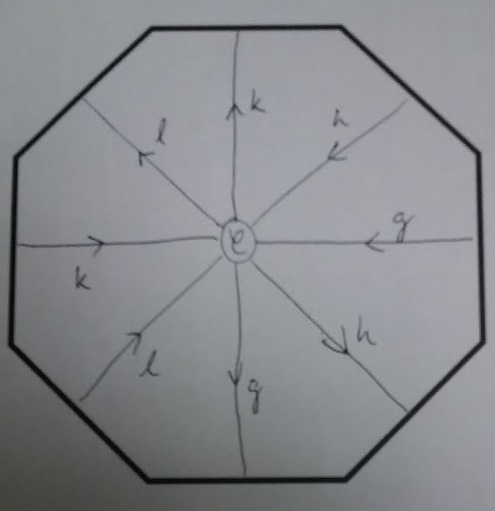
\includegraphics[width=0.5\textwidth]{basis.jpg}
\caption{Element of the spanning set $S$ for a genus 2 surface}
\label{fig:span}
\end{figure}

\begin{figure}
 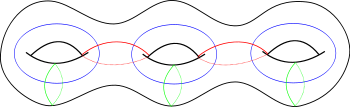
\includegraphics[width=.60\textwidth]{lickorish.png}
 \caption{Lickorish generating set (Image source: \url{https://en.wikipedia.org/wiki/Dehn_twist})}
\label{fig:lickorish}
\end{figure}


The mapping class group of $M$ is generated by the Lickorish generating set consisting of Dehn twists around $3g-1$ simple closed curves.  These can be divided into two types of twists: the ones around a single hole (the blue and green curves in Figure \ref{fig:lickorish}), and the ones connecting two holes (the red curves).

 Using the local moves as in Figures \ref{fig:tikzTwist1_1} to \ref{fig:tikzTwist2_5}, one sees that the result of each of these Dehn twists lies in $\Img(\omega) S$ since the structural morphisms of $\Vect_G^\omega$ have coefficients in $\Img(\omega)$.  It is a basic result in group cohomology that, by replacing $\omega$ with a cohomologous cocycle if necessary,  the image of $\omega$ lies in $\mu_{|G|}$, the set of $|G|$-th roots of unity.  Since cohomologous cocycles give rise to equivalent spherical categories $\Vect_G^\omega$, this replacement does not incur any loss in generality.

Thus, the image of any such mapping class group representation is a quotient of the group of permutations of the finite set $\mu_{|G|} S$, hence finite.
\end{proof}


\newcommand{\nc}{\newcommand}

%% Definitions

    % boundary of polygon
    % top left corner
     \nc{\lcx}{-0.5}
     \nc{\lcy}{0.866}
     \nc{\rcx}{-\lcx}
     \nc{\rcy}{\lcy}

     %TODO: Color edges
     \nc{\makeBdy}{
       \begin{scope}[very thick,decoration={
             markings,
             mark=at position 0.5 with {\arrow{>}}}
         ]  

         \draw(-1,0) -- (\lcx, \lcy); 
         \draw (\lcx, \lcy) -- (\rcx, \rcy); 
         \draw  (1, 0) -- (\rcx, \rcy);
       \end{scope}
     }

    %cut    
    % left endpoint of cut
    \nc{\lcutx}{-0.6}
    \nc{\lcuty}{0.6928}
    \nc{\lcut}{(\lcutx, \lcuty)}
    \nc{\rcutx}{-\lcutx}
    \nc{\rcuty}{\lcuty}
    \nc{\rcut}{(\rcutx, \rcuty)}

    %Main vertex
    \nc{\mvx}{0}
    \nc{\mvy}{0.2}
    \nc{\mv}{(\mvx, \mvy)}

    % outgoing edge
    \nc{\outEdge}{\draw[postaction={decorate}]  (0, 0) -- \mv node[pos=.5, right]{$hgh^{-1}$};}

    % middle of top edge of polygon
    \nc{\mtopx}{0}
    \nc{\mtopy}{0.866}
    \nc{\mtop}{(\mtopx, \mtopy)}

\begin{table}[h!]
\centering

\begin{tabular}{|c|c|}

\hline

%Dehn twist 1.1
    \begin{tikzpicture}[scale=5]    

      % boundary of polygon
      \makeBdy


    \begin{scope}[very thick,decoration={
    markings,
    mark=at position 0.5 with {\arrow{>}}}
    ]  

      % cut for Dehn twist
      \draw[loosely dashed] \lcut -- \rcut;
      

      %graph edges

      \draw[postaction={decorate}]   \mv -- (0.75, 0.433) node[pos=.5,sloped,above]{$h$};
      \draw[postaction={decorate}]   \mv -- \mtop node[pos=.5,left]{$g$};
      \draw[postaction={decorate}]  (-0.75, 0.433) -- \mv node[pos=.5,sloped,above]{$h$};
      \outEdge

    \end{scope}
    \end{tikzpicture}

&

%1.2
    \begin{tikzpicture}[scale=5]
    
    %boundary of polygon
      \makeBdy

    %graph edges
    \begin{scope}[very thick,decoration={
    markings,
    mark=at position 0.5 with {\arrow{>}}}
    ] 


        \draw[postaction={decorate}]   \mv -- (0.75, 0.433) node[pos=.5,sloped,above]{$h$};
        % old g
        % \draw[postaction={decorate}]   \rb -- (0, 0.866) node[pos=.5,left]{$g$};
        \draw[postaction={decorate}]  (-0.75, 0.433) -- \mv node[pos=.5,sloped,above]{$h$};
        \outEdge

        % new g
        \draw[postaction={decorate}]  \mv -- \rcut
        node[pos=.5,sloped,above]{$g$};
        \draw[postaction={decorate}]  \lcut -- \mtop
        node[pos=.5,sloped,below]{$g$};

    \end{scope}
    \end{tikzpicture}

\\ \hline

%1.3
      \begin{tikzpicture}[scale=5]
    
    %boundary of polygon
      \makeBdy

    %graph edges
    \begin{scope}[very thick,decoration={
    markings,
    mark=at position 0.5 with {\arrow{>}}}
    ] 

        \draw[postaction={decorate}]   \mv -- (0.75, 0.433) node[pos=.5,sloped,above]{$h$};
        \draw[postaction={decorate}]  (-0.75, 0.433) -- \mv node[pos=.5,sloped,above]{$h$};

        \outEdge

        \draw[postaction={decorate}]  \mv -- \rcut
        node[pos=.5,sloped,above]{$g$};
        %\draw[postaction={decorate}]  \lcut -- \mtop
        \draw[postaction={decorate}]  \lcut --  ({(\lcutx + \mtopx)/2} , {(\lcuty + \mtopy)/2})
        node[pos=.5,sloped,below]{$g$};
        \draw[postaction={decorate}]  ({(\lcutx + \mtopx)/2} , {(\lcuty + \mtopy)/2}) -- \mtop
        node[pos=.5,sloped,below]{$g$};


        \draw  \mv --  ({(\lcutx + \mtopx)/2} , {(\lcuty + \mtopy)/2});

    \end{scope}
    \end{tikzpicture}

&

%1.4
    
    \begin{tikzpicture}[scale=3]

      %boundary of polygon
      \makeBdy


      
      \begin{scope}[very thick,decoration={
            markings,
            mark=at position 0.5 with {\arrow{>}}}
        ] 
      %graph edges

        \draw[postaction={decorate}]   \mv -- (0.75, 0.433) node[pos=.5,sloped,above]{$h$};
        \draw[postaction={decorate}]  (-0.75, 0.433) -- \mv node[pos=.5,sloped,above]{$h$};

        \outEdge

        \draw[postaction={decorate}]  \mv -- \rcut
        node[pos=.5,sloped,above]{$g$};
        %\draw[postaction={decorate}]  \lcut -- \mtop
        \draw[postaction={decorate}]  \lcut -- \mv
        node[pos=.5,sloped,above]{$g$};
        \draw[postaction={decorate}]  \mv -- \mtop
        node[pos=.5,right]{$g$};


    \end{scope}
    \end{tikzpicture}

\\ \hline

%Dehn twist 1.5

    
    \begin{tikzpicture}[scale=5]

    % boundary of polygon
     \makeBdy
    
    %graph edges
    \begin{scope}[very thick,decoration={
    markings,
    mark=at position 0.5 with {\arrow{>}}}
    ]  
        \draw[postaction={decorate}]   \mv -- (0.75, 0.433) node[pos=.5,sloped,above]{$hg$};
        \draw[postaction={decorate}]   \mv -- \mtop node[pos=.5,left]{$g$};
        \draw[postaction={decorate}]  (-0.75, 0.433) -- \mv node[pos=.5,sloped,above]{$hg$};
        \outEdge

    \end{scope}
    \end{tikzpicture}
\\ \hline
\end{tabular}

\caption{First type of Dehn twist}
\label{fig:tikzTwist1_1}
\end{table}

%%%%%%%%%%%% Twist 2 %%%%%%%%%%%%%%%%


\nc{\makeBdyTwo}{
  \begin{scope}[very thick,decoration={
    markings,
    mark=at position 0.5 with {\arrow{>}}}
    ]  
    \path[draw]
    (1.0,          0.0) --       %0
    (0.92388,      0.382683)  -- %1
    (0.707107,     0.707107) --  %2
    (0.382683,     0.92388) --   %3
    (0,            1.0)   --     %4
    (-0.382683,    0.92388) --   %5
    (-0.707107 ,   0.707107)  -- %6
    ( -0.92388,    0.382683) --  %7
    ( -1.0     ,   0);           %8

  \end{scope}
}

\nc{\outEdgeTwo}{\draw[postaction={decorate}]  (0, 0) -- \mv node[pos=.5, right]{$[a,b][c,d]$};}

% 0.9 1 + 0.1 6
\nc{\cutOneX}{{0.8*(-0.92388) + 0.2*(-0.707107)}}
\nc{\cutOneY}{{0.8*(0.382683) + 0.2*(0.707107)}}
\nc{\cutOne}{(\cutOneX, \cutOneY)}

%0.9 3 + 0.1 4
\nc{\cutTwoX}{{0.8*(0.382683) + 0.2*(0)}}
\nc{\cutTwoY}{{0.8*(0.92388) + 0.2*(1.0)}}
\nc{\cutTwo}{(\cutTwoX, \cutTwoY)}

%0.9 2 + 0.1 1
\nc{\cutThreeX}{{0.8*(0.707107 ) + 0.2*(0.92388 )}}
\nc{\cutThreeY}{{0.8*(0.707107 ) + 0.2*(0.382638 )}}
\nc{\cutThree}{(\cutThreeX, \cutThreeY)}

%0.9 2 + 0.1 3
\nc{\cutFourX}{{0.2*( 0.382683) + 0.8*(0.707107)}}
\nc{\cutFourY}{{0.2*( 0.92388) + 0.8*(0.707107)}}
\nc{\cutFour}{(\cutFourX, \cutFourY)}

%0.1 0   0.9 1
\nc{\cutFiveX}{{0.2*( 1.0) + 0.8*(0.92388)}}
\nc{\cutFiveY}{{0.2*( 0.0) + 0.8*(0.382638)}}
\nc{\cutFive}{(\cutFiveX, \cutFiveY)}

%0.1 2   0.9 1
\nc{\cutSixX}{{0.2*( 0.707107) + 0.8*(0.92388)}}
\nc{\cutSixY}{{0.2*( 0.707107) + 0.8*(0.382683)}}
\nc{\cutSix}{(\cutSixX, \cutSixY)}

%0.1 3      0.9 4
\nc{\cutSevenX}{{0.2*( 0.382683) + 0.8*(0.0)}}
\nc{\cutSevenY}{{0.2*( 0.92388) + 0.8*(1.0)}}
\nc{\cutSeven}{(\cutSevenX, \cutSevenY)}

%0.1 5 0.9 4
\nc{\cutEightX}{{0.2*( -0.382683) + 0.8*(0.0)}}
\nc{\cutEightY}{{0.2*( 0.92388) + 0.8*(1.0)}}
\nc{\cutEight}{(\cutEightX, \cutEightY)}

\begin{figure}
    
    \begin{tikzpicture}[scale=8]

    % boundary of polygon
     \makeBdyTwo

     % cut for Dehn twist
     \draw[dotted] \cutOne -- \cutTwo;
     \draw[dotted] \cutThree -- \cutFour;
     \draw[dotted] \cutFive -- \cutSix;
     \draw[dotted] \cutSeven -- \cutEight;
         
    %graph edges
    \begin{scope}[very thick,decoration={
    markings,
    mark=at position 0.5 with {\arrow{>}}}
    ]  
       \draw[postaction={decorate}]  \mv -- (   0.96194 , 0.191342) node[pos=.5,sloped,above]{$a$};
       \draw[postaction={decorate}]  \mv -- ( 0.815493,  0.544895) node[pos=.5,sloped,above]{$b$};
       \draw[postaction={decorate}] (0.544895,  0.815493) -- \mv  node[pos=.5,sloped,above]{$a$};
       \draw[postaction={decorate}]   (0.191342,  0.96194) -- \mv  node[pos=.5,sloped,above]{$b$}; 
       \draw[postaction={decorate}]  \mv -- (-0.191342,  0.96194) node[pos=.5,sloped,above]{$c$}; 
       \draw[postaction={decorate}]  \mv -- (-0.544895,  0.815493) node[pos=.5,sloped,above]{$d$}; 
       \draw[postaction={decorate}] (-0.815493,  0.544895) -- \mv  node[pos=.5,sloped,above]{$c$};
       \draw[postaction={decorate}] (-0.96194,   0.191342) -- \mv  node[pos=.5,sloped,above]{$d$};

         \outEdgeTwo
    \end{scope}
    \end{tikzpicture}
    \caption{Second type of Dehn twist}
    \label{fig:tikzTwist2_0}
\end{figure}


\nc{\mvTwo}{ (-0.312076, 0.753418) }


\begin{figure}
    
    \begin{tikzpicture}[scale=8]

    % boundary of polygon
     \makeBdyTwo

     % cut for Dehn twist
     \draw[dotted] \cutOne -- \cutTwo;
     \draw[dotted] \cutThree -- \cutFour;
     \draw[dotted] \cutFive -- \cutSix;
     \draw[dotted] \cutSeven -- \cutEight;
         
    %graph edges
    \begin{scope}[very thick,decoration={
    markings,
    mark=at position 0.5 with {\arrow{>}}}
    ]  
       \draw[postaction={decorate}]  \mv -- \mvTwo node[pos=.5,sloped,above]{$g := b^{-1}cdc^{-1}$};

       \draw[postaction={decorate}]  \mv -- (   0.96194 , 0.191342) node[pos=.5,sloped,above]{$a$};
       \draw[postaction={decorate}]  \mv -- ( 0.815493,  0.544895) node[pos=.5,sloped,above]{$b$};
       \draw[postaction={decorate}] (0.544895,  0.815493) -- \mv  node[pos=.5,sloped,above]{$a$};
       \draw[postaction={decorate}]   (0.191342,  0.96194) -- \mvTwo  node[pos=.5,sloped,above]{$b$}; 
       \draw[postaction={decorate}]  \mvTwo -- (-0.191342,  0.96194) node[pos=.5,sloped,above]{$c$}; 
       \draw[postaction={decorate}]  \mvTwo -- (-0.544895,  0.815493) node[pos=.5,sloped,above]{$d$}; 
       \draw[postaction={decorate}] (-0.815493,  0.544895) -- \mvTwo  node[pos=.5,sloped,above]{$c$};
       \draw[postaction={decorate}] (-0.96194,   0.191342) -- \mv  node[pos=.5,sloped,above]{$d$};

         \outEdgeTwo
    \end{scope}
    \end{tikzpicture}
    \caption{Second type of Dehn twist}
    \label{fig:tikzTwist2_1}
\end{figure}

%2.2
\begin{figure}
    
    \begin{tikzpicture}[scale=8]

    % boundary of polygon
     \makeBdyTwo
         
    %graph edges
    \begin{scope}[very thick,decoration={
    markings,
    mark=at position 0.5 with {\arrow{>}}}
    ]  
       \draw[postaction={decorate}]  \mv -- \cutTwo node[pos=.5,sloped,above]{$g$};
       \draw[postaction={decorate}]  \cutOne -- \mvTwo node[pos=.5,sloped,below]{$g$};
       \draw[postaction={decorate}]  \cutThree -- \cutFour node[pos=.5,sloped,below]{$g$};
       \draw[postaction={decorate}]  \cutFive -- \cutSix node[pos=.5,sloped,below]{$g$};
       \draw[postaction={decorate}]  \cutSeven -- \cutEight node[pos=.5,sloped,below]{$g$};


       \draw[postaction={decorate}]  \mv -- (   0.96194 , 0.191342) node[pos=.5,sloped,above]{$a$};
       \draw[postaction={decorate}]  \mv -- ( 0.815493,  0.544895) node[pos=.5,sloped,above]{$b$};
       \draw[postaction={decorate}] (0.544895,  0.815493) -- \mv  node[pos=.5,sloped,above]{$a$};
       \draw[postaction={decorate}]   (0.191342,  0.96194) -- \mvTwo  node[pos=.5,sloped,above]{$b$}; 
       \draw[postaction={decorate}]  \mvTwo -- (-0.191342,  0.96194) node[pos=.5,sloped,above]{$c$}; 
       \draw[postaction={decorate}]  \mvTwo -- (-0.544895,  0.815493) node[pos=.5,sloped,above]{$d$}; 
       \draw[postaction={decorate}] (-0.815493,  0.544895) -- \mvTwo  node[pos=.5,sloped,above]{$c$};
       \draw[postaction={decorate}] (-0.96194,   0.191342) -- \mv  node[pos=.5,sloped,above]{$d$};

         \outEdgeTwo
    \end{scope}
    \end{tikzpicture}
    \caption{Second type of Dehn twist}
    \label{fig:tikzTwist2_2}
\end{figure}


%2.3
\begin{figure}
    
    \begin{tikzpicture}[scale=8]

    % boundary of polygon
     \makeBdyTwo
         
    %graph edges
    \begin{scope}[very thick,decoration={
    markings,
    mark=at position 0.5 with {\arrow{>}}}
    ]  
       \draw[postaction={decorate}]  \mv -- \cutTwo node[pos=.5,sloped,above]{$g$};
       \draw[postaction={decorate}]  \cutThree -- \mv node[pos=.5,sloped,above]{$g$};

       \draw[postaction={decorate}]  \mv -- ( 0.96194 , 0.191342) node[pos=.5,sloped,above]{$ag^{-1}$};
       \draw[postaction={decorate}]  \mv -- ( 0.815493,  0.544895) node[pos=.5,sloped,below]{$gb$};
       \draw[postaction={decorate}] (0.544895,  0.815493) -- \mv  node[pos=.5,sloped,above]{$ag^{-1}$};
       \draw[postaction={decorate}]   (0.191342,  0.96194) -- \mvTwo  node[pos=.5,sloped,above]{$gb$}; 
       \draw[postaction={decorate}]  \mvTwo -- (-0.191342,  0.96194) node[pos=.5,sloped,above]{$gc$}; 
       \draw[postaction={decorate}]  \mvTwo -- (-0.544895,  0.815493) node[pos=.5,sloped,above]{$d$}; 
       \draw[postaction={decorate}] (-0.815493,  0.544895) -- \mvTwo  node[pos=.5,sloped,above]{$gc$};
       \draw[postaction={decorate}] (-0.96194,   0.191342) -- \mv  node[pos=.5,sloped,above]{$d$};

         \outEdgeTwo
    \end{scope}
    \end{tikzpicture}
    \caption{Second type of Dehn twist}
    \label{fig:tikzTwist2_3}
\end{figure}

%2.4
\begin{figure}
    
    \begin{tikzpicture}[scale=8]

    % boundary of polygon
     \makeBdyTwo
         
    %graph edges
    \begin{scope}[very thick,decoration={
    markings,
    mark=at position 0.5 with {\arrow{>}}}
    ]  
       \draw[postaction={decorate}]  \mv -- \cutTwo node[pos=.5,sloped,below]{$g$};
       \draw[postaction={decorate}]  \cutThree -- \mv node[pos=.5,sloped,above]{$g$};

       \draw[postaction={decorate}]  \mv -- ( 0.96194 , 0.191342) node[pos=.5,sloped,above]{$ag^{-1}$};
       \draw[postaction={decorate}]  \mv -- ( 0.815493,  0.544895) node[pos=.5,sloped,below]{$gb$};
       \draw[postaction={decorate}] (0.544895,  0.815493) -- \mv  node[pos=.5,sloped,above]{$ag^{-1}$};
       \draw[postaction={decorate}]   (0.191342,  0.96194) -- \mv  node[pos=.5,sloped,above]{$gb$}; 
       \draw[postaction={decorate}]  \mv -- (-0.191342,  0.96194) node[pos=.5,sloped,above]{$gc$}; 
       \draw[postaction={decorate}]  \mv -- (-0.544895,  0.815493) node[pos=.5,sloped,above]{$d$}; 
       \draw[postaction={decorate}] (-0.815493,  0.544895) -- \mv  node[pos=.5,sloped,above]{$gc$};
       \draw[postaction={decorate}] (-0.96194,   0.191342) -- \mv  node[pos=.5,sloped,above]{$d$};

         \outEdgeTwo
    \end{scope}
    \end{tikzpicture}
    \caption{Second type of Dehn twist}
    \label{fig:tikzTwist2_4}
\end{figure}

%2.5
\begin{figure}
    
    \begin{tikzpicture}[scale=8]

    % boundary of polygon
     \makeBdyTwo
         
    %graph edges
    \begin{scope}[very thick,decoration={
    markings,
    mark=at position 0.5 with {\arrow{>}}}
    ]  

       \draw[postaction={decorate}]  \mv -- ( 0.96194 , 0.191342) node[pos=.5,sloped,above]{$ag^{-1}$};
       \draw[postaction={decorate}]  \mv -- ( 0.815493,  0.544895) node[pos=.5,sloped,above]{$gbg^{-1}$};
       \draw[postaction={decorate}] (0.544895,  0.815493) -- \mv  node[pos=.5,sloped,above]{$ag^{-1}$};
       \draw[postaction={decorate}]   (0.191342,  0.96194) -- \mv  node[pos=.5,sloped,above]{$gbg^{-1}$}; 
       \draw[postaction={decorate}]  \mv -- (-0.191342,  0.96194) node[pos=.5,sloped,above]{$gc$}; 
       \draw[postaction={decorate}]  \mv -- (-0.544895,  0.815493) node[pos=.5,sloped,above]{$d$}; 
       \draw[postaction={decorate}] (-0.815493,  0.544895) -- \mv  node[pos=.5,sloped,above]{$gc$};
       \draw[postaction={decorate}] (-0.96194,   0.191342) -- \mv  node[pos=.5,sloped,above]{$d$};

         \outEdgeTwo
    \end{scope}
    \end{tikzpicture}
    \caption{Second type of Dehn twist}
    \label{fig:tikzTwist2_5}
\end{figure}

\section{Example Calculation}
This section contains a calculation of the coefficient for the first Dehn twist shown in Figure \ref{fig:tikzTwist1_1}.   Assume that the main vertex is initially labeled with an element of $\Hom(1, h \otimes g \otimes 1 \otimes h^{-1} \otimes hg^{-1}h^{-1})$.   In the following, we will abbreviate by saying that the vertex is in state $h \otimes g \otimes 1 \otimes h^{-1} \otimes hg^{-1}h^{-1}$.

In Figure \ref{fig:tikzTwist1_3}, we add the upper left vertex, which is labeled by  $\coev_g$.  We then connect the vertices with an unlabelled edge, which is shorthand for labelling by the object $1$ .  At this point, the vertices are in states $h \otimes g \otimes 1 \otimes h^{-1} \otimes hg^{-1}h^{-1}$ and $g \otimes g^{-1}  \otimes 1$.  To compose the two vertices, we use the spherical structure on the former vertex and reassociate until it is in the state $h^{-1} \otimes h g^{-1} h^{-1} \otimes h \otimes g \otimes 1$.  In doing so, we pick up a factor of 
$$ \omega(h, g, h^{-1}) \omega(h, gh^{-1}, hg^{-1}h^{-1}) \omega(g, h^{-1}, hg^{-1}h^{-1}) \omega(g, g^{-1}h^{-1}, h) $$
% $$\omega^{-1}(hg^{-1}h^{-1}, hg, h^{-1}) \omega^{-1}(hg^{-1}h^{-1}, h, g) \omega^{-1}(h^{-1}, hg^{-1}, g) \omega^{-1}(h^{-1}, hg^{-1}h^{-1}, h) $$

After performing the composition, we are in the situation of Figure $\ref{fig:tikzTwist1_4}$ with state $h^{-1} \otimes hg^{-1}h^{-1} \otimes h \otimes g \otimes (g \otimes g^{-1})$.  To get rid of the last pair of parentheses, we get a factor of $\omega^{-1}(h^{-1}hg^{-1}h^{-1}hg, g, g^{-1}) = \omega^{-1}(1, g, g^{-1}) = 1$.   

To tensor the parallel $g$ and $h$ edges together, we add $\coev_g$ and $\coev_h$ vertices in the middle of those edges and connect them with a $1$.  Composing along the $1$, we get a vertex in state $g \otimes g^{-1} \otimes h^{-1} \otimes h$.  To put this vertex in state $g^{-1}h^{-1} \otimes hg$ we pick up a factor of $\omega(g, g^{-1}, h^{-1}) \omega(g, g^{-1}h^{-1}, h) \omega(g^{-1}h^{-1}, h, g)$.   We also put the original vertex in the state $g^{-1}h^{-1} \otimes hg^{-1}h^{-1} \otimes hg \otimes g$ with a factor of
$$\omega^{-1}(g^{-1}, g^{-1}, g) \omega^{-1}(g^{-1}, g^{-1}h^{-1}, h) \omega^{-1}(g^{-1}, h^{-1}, hg^{-1}h^{-1}) \omega(g^{-2}h^{-1}, h, g). $$

To compose the two vertices, we rotate the original vertex to the state $g  \otimes g^{-1}h^{-1}  \otimes hg^{-1}h^{-1} \otimes hg$ which yields a factor of 
$$\omega^{-1}(g, h^{-1}, hg) \omega^{-1}(g, g^{-1}h^{-1}, hg^{-1}h^{-1}) \omega^{-1}(g, g^{-1}, h^{-1}).$$
We are then in a position to compose the two vertices, giving a factor 
$\omega(g^{-1}h^{-1}, hg, g^{-1}h^{-1})  \ev_{g^{-1}h^{-1}} = 1$ and a vertex in state $g \otimes g^{-1}h^{-1} \otimes hg^{-1}h^{-1} \otimes hg$.  Rotating the vertex into its initial configuration $hg \otimes g \otimes  g^{-1}h^{-1} \otimes hg^{-1}h^{-1}$ gives a factor 
of 
$$\omega^{-1}(hg, h^{-1}, hg^{-1}h^{-1}) \omega^{-1}(hg, g, g^{-1}h^{-1}).$$

 Thus, we have an overall factor of
{\allowdisplaybreaks
\begin{align*} 
&  \frac{\omega(h, g, h^{-1}) \omega(h, gh^{-1}, hg^{-1}h^{-1}) \omega(g, h^{-1}, hg^{-1}h^{-1}) \omega(g, g^{-1}h^{-1}, h) } 
{\omega(g^{-1}, g^{-1}, g) \omega(g^{-1}, g^{-1}h^{-1}, h) \omega(g^{-1}, h^{-1}, hg^{-1}h^{-1})  \omega(g, g^{-2}h^{-1}, hg)} \cdot \\ 
& \qquad  \frac{\omega(g, g^{-1}, h^{-1}) \omega(g, g^{-1}h^{-1}, h) \omega(g^{-1}h^{-1}, h, g) \omega(g^{-2}h^{-1}, h, g)}
{\omega(g, g^{-1}h^{-1}, hg^{-1}h^{-1}) \omega(hg, h^{-1}, hg^{-1}h^{-1}) \omega(hg, g, g^{-1}h^{-1})} \\
& = \frac{\omega(h, g, g^{-1}h^{-1})\omega(g, g^{-1}h^{-1}, h) } 
{\omega(g^{-1}, g^{-1}, g) \omega(g^{-1}, g^{-1}h^{-1}, h) \omega(g^{-1}, h^{-1}, hg^{-1}h^{-1})  \omega(g, g^{-2}h^{-1}, hg)} \cdot \\ 
& \qquad \frac{\omega(g, g^{-1}, h^{-1}) \omega(g, g^{-1}h^{-1}, h) \omega(g^{-1}h^{-1}, h, g) \omega(g^{-2}h^{-1}, h, g)}
{\omega(g, g^{-1}h^{-1}, hg^{-1}h^{-1}) \omega(hg, g, g^{-1}h^{-1}) } \\
& = \frac{\omega(h, g, g^{-1}h^{-1})\omega(g, g^{-1}h^{-1}, h) } 
{\omega(g^{-1}, g^{-1}, g) \omega(g^{-1}, g^{-1}h^{-1}, h)  \omega(g, g^{-2}h^{-1}, hg)} \cdot \\ 
& \qquad \frac{\omega^2(g, g^{-1}, h^{-1}) \omega(g, g^{-1}h^{-1}, h) \omega(g^{-1}h^{-1}, h, g) \omega(g^{-2}h^{-1}, h, g)}
{\omega(g, g^{-1}, g^{-1}h^{-1}) \omega(hg, g, g^{-1}h^{-1}) } \\
& = \frac{\omega(h, g, g^{-1}h^{-1})\omega^2(g, g^{-1}h^{-1}, h) \omega^2(g, g^{-1}, h^{-1})  \omega^2(g^{-1}h^{-1}, h, g)} 
{ \omega(g, g^{-2}h^{-1}, hg) \omega(g, g^{-1}, g^{-1}h^{-1}) \omega(hg, g, g^{-1}h^{-1}) \omega(g^{-1}, g^{-1}h^{-1}, hg)} \\
& = \frac{\omega(h, g, g^{-1}h^{-1})\omega^2(g, g^{-1}h^{-1}, h) \omega^2(g, g^{-1}, h^{-1}) \omega^2(g^{-1}h^{-1}, h, g) } 
{  \omega(hg, g, g^{-1}h^{-1}) } \\
& = \frac{\omega(h, g, g^{-1}h^{-1})  \omega^2(g^{-1}h^{-1}, h, g) } 
{\omega^2(g^{-1}, h^{-1},h)  \omega(hg, g, g^{-1}h^{-1}) } 
\end{align*}
}


\section{Further Directions}
Given the fact that the braid group representations associated to $D^\omega(G)$ are also finite \cite{erw}, it should  be possible
 to prove that mapping class group representations associated to $\Vect^\omega(G)$ for any orientable surface, including boundary, are finite.  
The basic idea is that one labels the boundary components with elements of the double category, in this case $\Mod(D^\omega(G))$, and the
$\Vect_G^\omega$-colored embedded graphs must be compatible with the boundary labels, as detailed in \cite{kirillovStringNets}.  

One could also consider more complicated spherical categories than $\Vect^\omega(G)$, such as the 
Tambara-Yamagami categories.  The main additional complication here is the appearance of multiplicity, i.e. the tensor product of 
two simple objects can be a direct sum of multiple simple objects.  
\medskip


 
\bibliographystyle{unsrt}
\bibliography{stringnets}



\end{document}
